\documentclass[12pt, twoside]{article}
\usepackage[letterpaper, margin=1in, headsep=0.5in]{geometry}
\usepackage[english]{babel}
\usepackage[utf8]{inputenc}
\usepackage{amsmath}
\usepackage{amsfonts}
\usepackage{amssymb}
\usepackage{tikz}
\usetikzlibrary{quotes, angles}
\usepackage{graphicx}
\usepackage{enumitem}
\usepackage{multicol}
\usepackage{hyperref}

\newif\ifmeta
\metatrue %print standards and topics tags

\title{IB Mathematics}
\author{Chris Huson}
\date{September 2021}

\usepackage{fancyhdr}
\pagestyle{fancy}
\fancyhf{}
\renewcommand{\headrulewidth}{0pt} % disable the underline of the header
\raggedbottom


\fancyhead[LE]{\thepage}
\fancyhead[RO]{\thepage \\ Name: \hspace{4cm} \,\\}
\fancyhead[LO]{BECA / IB Math 01-Linear functions\\* 7 October 2021}

\begin{document}

\subsubsection*{PreQuiz: I can model with linear functions}
Equations of a straight line: $f(x)=mx+c$, $ax+by+d=0$, $(y-y_1)=m(x-x_1)$\\[0.25cm]
Gradient: $\displaystyle m=\frac{y_2-y_1}{x_2-x_1}$ \vspace{1cm}
\begin{enumerate}
\item A linear function $f$ is graphed below.
\begin{multicols}{2}
\begin{enumerate}
  \item Write down it's slope.\\ $m=$
  \vspace{0.25cm}
  \item Write down it's $y$-intercept.\\ $b=$
  \vspace{0.25cm}
  \item Write down the equation of the line.
  \vspace{1cm}
  \item State the coordinates of the point $P$.
\end{enumerate} \vspace{.5cm}
  \begin{center} 
  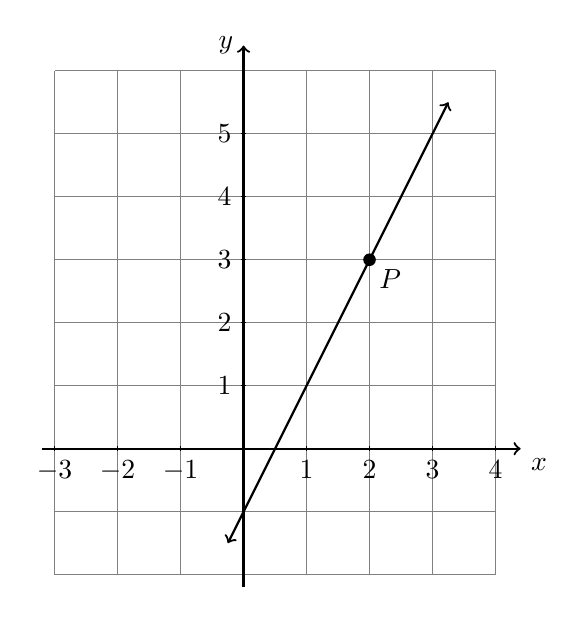
\begin{tikzpicture}[scale=0.8]
    \draw [help lines] (-3,-2) grid (4,6);
    \draw [thick, ->] (-3.2,0) -- (4.4,0) node [below right] {$x$};
    \draw [thick, ->] (0,-2.2)--(0,6.4) node [left] {$y$};
    \foreach \x in {-3,-2,-1,1,2,...,4} \draw (\x cm,1pt) -- (\x cm,-1pt) node[anchor=north] {$\x$};
    \foreach \y in {1, 2, 3, 4, 5} \draw (1pt,\y cm) -- (-1pt,\y cm) node[anchor=east] {$\y$};
    \draw [thick, <->] (-0.25,-1.5) -- (3.25,5.5);
    \fill (2,3) circle[radius=0.1] node[below right]{$P$};
  \end{tikzpicture}
  \end{center}
\end{multicols}

\item Write the linear equation $y-2=3(x+1)$ in the form $y=mx+c$. \vspace{4cm}

\item A line has a gradient (slope) of 3 and goes through the point $(1, 4)$. Find the equation of the line in the form $y=mx+b$.

\newpage
\item A line goes through the points $(2, 10)$ and $(5, 18)$. Find the gradient and the equation of the line in the form $y=mx+b$.

\begin{enumerate}
  \begin{multicols}{2}
      \item Find the gradient of the line.
      \item Find the equation of the line.\vspace{2cm}
      \begin{center}
      \begin{tikzpicture}[xscale=0.7, yscale=0.4]
        %\draw [help lines] (-3,-2) grid (4,6);
        \draw [thick, ->] (-1.2,0) -- (7.4,0) node [below right] {$x$};
        \draw [thick, ->] (0,-1.2)--(0,13.5) node [right] {$y$};
        \foreach \x in {-1, 1,2, ..., 7} \draw (\x cm,4pt) -- (\x cm,-4pt) node[anchor=north] {$\x$};
        \foreach \y in {2, 4, ..., 12} \draw (2pt,\y cm) -- (-2pt,\y cm) node[anchor=east] {$\y$};
      \end{tikzpicture}
      \end{center}
    \end{multicols}
\end{enumerate}

\item Find the equation of the line through the points $(-2, 5)$ and $(3,  20)$. 

  \newpage
  \item A function $f$ is shown in the table. \hfill [5]
  \begin{center}
    \begin{tabular}{|l|r|r|r|r|r|r|}
      \hline
      $x$ & 0 & 2 & 4 & 6 & 8\\ 
      \hline 
      $f(x)$ & 0 & 1 & 2 & 3 & 4\\ 
      \hline 
    \end{tabular}
  \end{center}
  \begin{enumerate}[itemsep=2.5cm]
    \item Is $f$ a linear function? Why or why not?
    \item Is $f$ a direct variation? Explain.
    \item Find the gradient of the function. \vspace{1cm}
    \item Write down the equation of $f$ in the form $y=mx+c$
    \item Complete the table of the inverse of $f$.
      \begin{center}
        \begin{tabular}{|l|r|r|r|r|r|r|}
          \hline
          $x$ & \hspace{1cm} & \hspace{1cm} & \hspace{1cm} & \hspace{1cm} & \hspace{1cm}.\\[1cm] 
          \hline 
          $f^{-1}(x)$ & \hspace{1cm} & \hspace{1cm} & \hspace{1cm} & \hspace{1cm} & \hspace{1cm}.\\[1cm] 
          \hline 
        \end{tabular}
      \end{center}
  \end{enumerate}

\newpage
\item A linear function is such that $f(1)=5$ and $f(5)=1$.
\begin{enumerate}[itemsep=1.5cm]
  \item Name two of the function's points as ordered pairs.
  \item Find the gradient (slope) for the function $f$
  \item Substitute the slope and one point into the formula $f(x)=mx+c$
  \item Solve for the $y$-intercept
  \item Find $f(-3)$
\end{enumerate} \vspace{1cm}

\item Given the direct variation (and also a linear function) $f(x)=2x$. \hfill [6]
\begin{enumerate}
  \begin{multicols}{2}
    \item Find $f(3)$
    \item   $f(x)=10$. Find $x$.
  \end{multicols}\vspace{2cm}
  \begin{multicols}{2}
      \item Plot the answers to the first two parts, (a) and (b), as points on the grid and label them as ordered pairs. 
      \item Draw a straight line through the points to represent the function.
      \item What is the constant of proportionality? \vspace{2cm}
      \begin{center}
      \begin{tikzpicture}[xscale=0.7, yscale=0.4]
        %\draw [help lines] (-3,-2) grid (4,6);
        \draw [thick, ->] (-1.2,0) -- (7.4,0) node [below right] {$x$};
        \draw [thick, ->] (0,-1.2)--(0,13.5) node [right] {$y$};
        \foreach \x in {-1, 1,2, ..., 7} \draw (\x cm,4pt) -- (\x cm,-4pt) node[anchor=north] {$\x$};
        \foreach \y in {2, 4, ..., 12} \draw (2pt,\y cm) -- (-2pt,\y cm) node[anchor=east] {$\y$};
      \end{tikzpicture}
      \end{center}
    \end{multicols}
\end{enumerate}

\item The gasoline used by a car is the function of the distance driven in miles, as shown in the table.
\begin{center}
  \begin{tabular}{|l|r|r|r|r|r|r|}
    \hline
    Distance (miles) & 10 & 20 & 40 & 50 & 200 & 500\\ 
    \hline 
    Gas (gallons) & 0.5 & 1 & 2 & 2.5 & 10 & 25\\ 
    \hline 
  \end{tabular}
\end{center}
\begin{enumerate}[itemsep=1cm]
  \item Is gas usage a linear function of distance driven? Explain.
  \item Is it a direct variation?
  \item What is the gradient? 
  \item What is the gas mileage in terms of miles per gallon?
  \item Discuss which is the independent and dependent variables.
\end{enumerate}

\end{enumerate}
\end{document}